\documentclass[tikz,border=6pt]{standalone}
\usepackage[T1]{fontenc}
\usepackage{lmodern}
\usepackage{amsmath}
\usepackage{pgfplots}
\pgfplotsset{compat=1.18}
\usetikzlibrary{arrows.meta,positioning,fit,backgrounds,shapes.geometric,calc}
\definecolor{navy}{HTML}{16324F}
\definecolor{tealC}{HTML}{007F82}
\definecolor{amberC}{HTML}{D97706}
\definecolor{coralC}{HTML}{C2410C}
\definecolor{redC}{HTML}{DC2626}
\definecolor{mintC}{HTML}{059669}
\definecolor{slateC}{HTML}{64748B}
\definecolor{paleBg}{HTML}{F4F7FA}
\definecolor{softTeal}{HTML}{E6F4F4}
\definecolor{softNavy}{HTML}{EAF0F6}
\definecolor{softAmber}{HTML}{FEF3C7}
\begin{document}

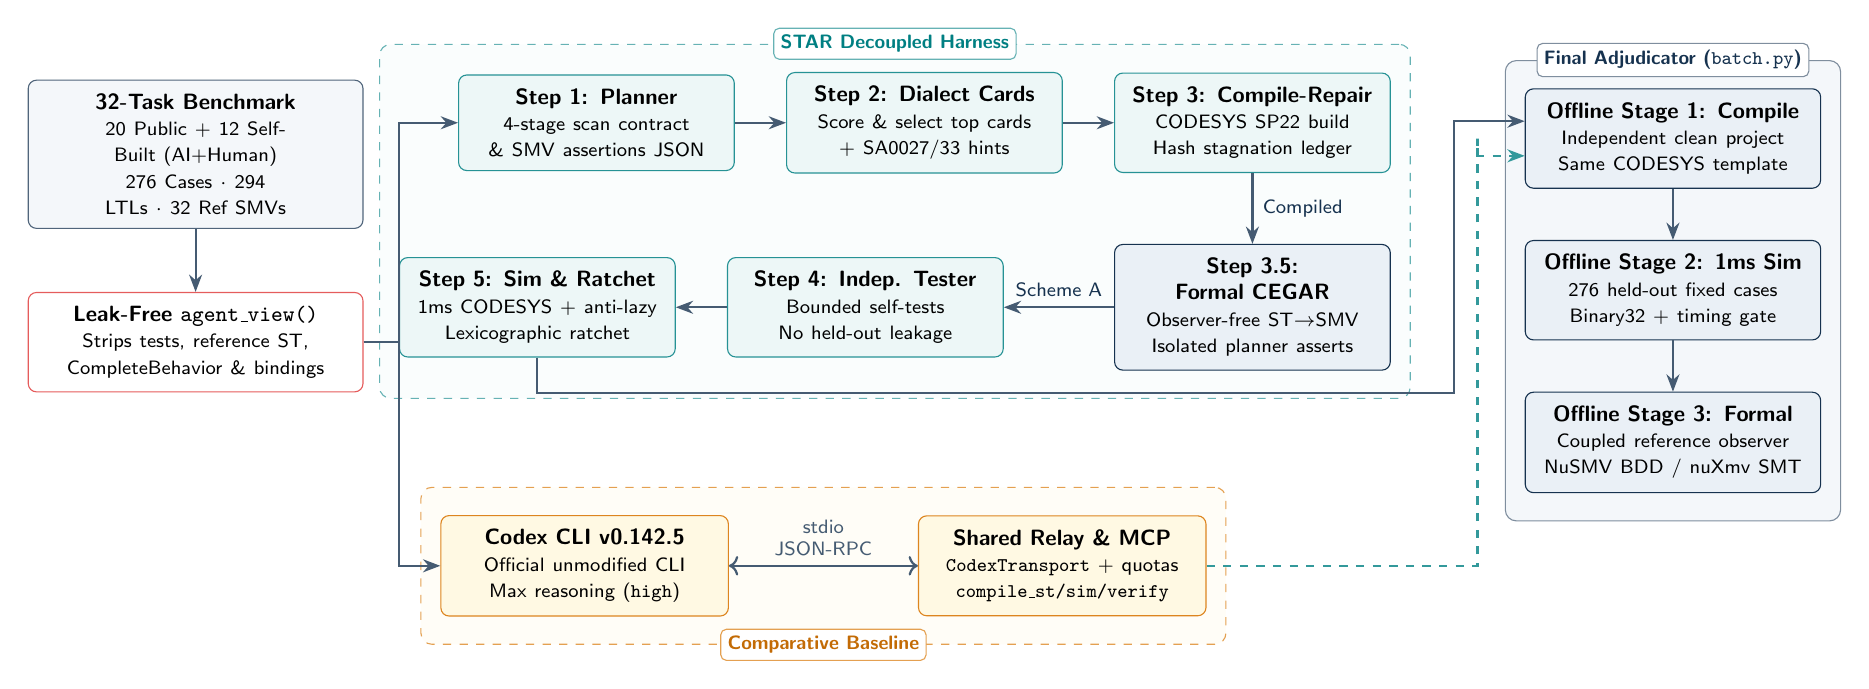
\begin{tikzpicture}[
    node distance=7mm and 9mm,
    font=\sffamily\footnotesize,
    box/.style={draw=navy!75, rounded corners=3pt, fill=white, align=center, inner sep=5pt, minimum height=9.5mm},
    stage/.style={box, draw=tealC!85, fill=softTeal!70, text width=31.5mm},
    base/.style={box, draw=amberC!90, fill=softAmber!50, text width=33mm},
    eval/.style={box, draw=navy, fill=softNavy, text width=34mm},
    arr/.style={-{Stealth[length=2.2mm]}, thick, color=navy!80},
    dasharr/.style={-{Stealth[length=2.2mm]}, thick, dashed, color=tealC!80}
]

% Benchmark Dataset & Agent View
\node[box, fill=paleBg, text width=39mm] (db) {\textbf{32-Task Benchmark}\\{\scriptsize 20 Public + 12 Self-Built (AI+Human)}\\{\scriptsize 276 Cases $\cdot$ 294 LTLs $\cdot$ 32 Ref SMVs}};
\node[box, fill=white, draw=redC!75, below=8mm of db, text width=39mm] (view) {\textbf{Leak-Free \texttt{agent\_view()}}\\{\scriptsize Strips tests, reference ST,}\\{\scriptsize CompleteBehavior \& bindings}};

\draw[arr] (db) -- (view);

% STAR Pipeline (Upper Branch)
\node[stage, right=12mm of db, yshift=4mm] (s1) {\textbf{Step 1: Planner}\\{\scriptsize 4-stage scan contract}\\{\scriptsize \& SMV assertions JSON}};
\node[stage, right=6.5mm of s1] (s2) {\textbf{Step 2: Dialect Cards}\\{\scriptsize Score \& select top cards}\\{\scriptsize + SA0027/33 hints}};
\node[stage, right=6.5mm of s2] (s3) {\textbf{Step 3: Compile-Repair}\\{\scriptsize CODESYS SP22 build}\\{\scriptsize Hash stagnation ledger}};
\node[stage, below=9mm of s3, fill=softNavy, draw=navy] (s35) {\textbf{Step 3.5:}\\\textbf{Formal CEGAR}\\{\scriptsize Observer-free ST$\to$SMV}\\{\scriptsize Isolated planner asserts}};
\node[stage, left=14mm of s35] (s4) {\textbf{Step 4: Indep. Tester}\\{\scriptsize Bounded self-tests}\\{\scriptsize No held-out leakage}};
\node[stage, left=6.5mm of s4] (s5) {\textbf{Step 5: Sim \& Ratchet}\\{\scriptsize 1ms CODESYS + anti-lazy}\\{\scriptsize Lexicographic ratchet}};

\draw[arr] (view.east) -- ++(4.5mm,0) |- (s1.west);
\draw[arr] (s1) -- (s2);
\draw[arr] (s2) -- (s3);
\draw[arr] (s3) -- node[right, font=\sffamily\scriptsize, color=navy] {Compiled} (s35);
\draw[arr] (s35) -- node[above, font=\sffamily\scriptsize, color=navy] {Scheme A} (s4);
\draw[arr] (s4) -- (s5);

% Codex Baseline (Lower Branch)
\node[base, below=20mm of s5, xshift=6mm] (codex) {\textbf{Codex CLI v0.142.5}\\{\scriptsize Official unmodified CLI}\\{\scriptsize Max reasoning (\texttt{high})}};
\node[base, right=24mm of codex] (mcp) {\textbf{Shared Relay \& MCP}\\{\scriptsize \texttt{CodexTransport} + quotas}\\{\scriptsize \texttt{compile\_st/sim/verify}}};

\draw[arr] (view.east) -- ++(4.5mm,0) |- (codex.west);
\draw[arr, <->] (codex.east) -- node[above, font=\sffamily\scriptsize, align=center] {stdio\\JSON-RPC} (mcp.west);

% Offline Held-Out Final Evaluator (Right)
\node[eval, right=17mm of s3, yshift=-2mm] (e1) {\textbf{Offline Stage 1: Compile}\\{\scriptsize Independent clean project}\\{\scriptsize Same CODESYS template}};
\node[eval, below=6.5mm of e1] (e2) {\textbf{Offline Stage 2: 1ms Sim}\\{\scriptsize 276 held-out fixed cases}\\{\scriptsize Binary32 + timing gate}};
\node[eval, below=6.5mm of e2] (e3) {\textbf{Offline Stage 3: Formal}\\{\scriptsize Coupled reference observer}\\{\scriptsize NuSMV BDD / nuXmv SMT}};

\draw[arr] (s5.south) -- ++(0,-4.5mm) -| ($(e1.west)-(9mm,0)$) |- ([yshift=2.2mm]e1.west);
\draw[dasharr] (mcp.east) -| ($(e1.west)-(6mm,0)$) |- ([yshift=-2.2mm]e1.west);
\draw[arr] (e1) -- (e2);
\draw[arr] (e2) -- (e3);

\begin{scope}[on background layer]
  \node[draw=tealC!60, dashed, rounded corners=4pt, fill=softTeal!22, fit=(s1)(s2)(s3)(s35)(s4)(s5), inner xsep=7pt, inner ysep=10pt] (gstar) {};
  \node[draw=tealC!60, fill=white, rounded corners=2pt, inner sep=2.5pt, font=\sffamily\bfseries\scriptsize, text=tealC] at (gstar.north) {STAR Decoupled Harness};

  \node[draw=amberC!70, dashed, rounded corners=4pt, fill=softAmber!15, fit=(codex)(mcp), inner xsep=7pt, inner ysep=10pt] (gbase) {};
  \node[draw=amberC!70, fill=white, rounded corners=2pt, inner sep=2.5pt, font=\sffamily\bfseries\scriptsize, text=amberC!90!black] at (gbase.south) {Comparative Baseline};

  \node[draw=navy!55, rounded corners=4pt, fill=paleBg, fit=(e1)(e2)(e3), inner xsep=7pt, inner ysep=10pt] (geval) {};
  \node[draw=navy!55, fill=white, rounded corners=2pt, inner sep=2.5pt, font=\sffamily\bfseries\scriptsize, text=navy] at (geval.north) {Final Adjudicator (\texttt{batch.py})};
\end{scope}

\end{tikzpicture}
\end{document}
